\documentclass[aspectratio=169,10pt]{beamer}
\usepackage{common/pdmtheme}
\graphicspath{{figures/}}
\title[RA8D1 node]{Renesas EK-RA8D1}
\subtitle{Three axes, a real tachometer, and what speed does \emph{not} buy}
\author{Predictive Maintenance Platform}
\date{14 October 2026}
\begin{document}

\begin{frame}[plain]
  \vspace{5mm}
  {\LARGE\bfseries Renesas EK-RA8D1}\\[2mm]
  {\large\color{pdmink2} Three axes, a real tachometer, and what speed does
   \emph{not} buy}\par
  \vspace{5mm}\noindent{\color{pdmrule}\rule{\linewidth}{0.4pt}}\par
  \vspace{3mm}
  \begin{columns}[T]
    \begin{column}{0.46\textwidth}
      \scriptsize
      \kv{Core}{Cortex-M85 480 MHz, Helium MVE}\\[1mm]
      \kv{SRAM}{\textbf{1 MB} --- the real differentiator}\\[1mm]
      \kv{Pipeline}{1.3 ms per axis, 5.9 ms for three}\\[1mm]
      \kv{Tacho}{hardware capture --- the only kit with one}\\[1mm]
      \kv{Compute share}{8.8 \% of the energy cycle}\\[1mm]
      \kv{Battery life}{3.12 y (18650, self-discharge bound)}
    \end{column}
    \begin{column}{0.46\textwidth}
      \scriptsize\color{pdmink2}
      \textbf{Never flashed.} No Renesas toolchain in this environment, so the
      driver is compiled against a \emph{stub} FSP under the real warning set
      --- which proves its types and signatures, and not one register value.
      \\[2mm]
      The kit's distinctive module, angular resampling, \textbf{is} measured:
      14 checks on a synthetic swept-speed signal. The measurement
      contradicted the design's own assumption, which is this deck's main
      finding.
    \end{column}
  \end{columns}
  \srcnote{Branch \texttt{hw/renesas-ra8d1-helium}. 19 config property tests,
  14 order-tracking checks, 4 three-axis end-to-end tests, 1\,113 shared DSP
  checks.}
\end{frame}

% ------------------------------------------------------------ speed is a trap -
\begin{frame}{A faster core does not save energy}
  \centering
  \scriptsize
  \begin{tabular}{@{}lrrrr@{}}
    \toprule
    & \textbf{Clock} & \textbf{Pipeline} & \textbf{Current} & \textbf{Energy} \\
    \midrule
    STM32U585 (M33)            & 160 MHz & 8.6 ms & 21 mA & 0.18 mA$\cdot$s \\
    Alif E7 (M55 HE + Helium)  & 160 MHz & 2.4 ms & 9 mA  & 0.02 mA$\cdot$s \\
    \textbf{RA8D1 (M85 + Helium)} & \textbf{480 MHz} & \textbf{1.3 ms} &
      \textbf{62 mA} & \textbf{0.08 mA$\cdot$s} \\
    \midrule
    \textcolor{pdmcrit}{\textbf{Acquisition window}} & &
      \textcolor{pdmcrit}{\textbf{307 ms}} & \textcolor{pdmcrit}{\textbf{6 mA}} &
      \textcolor{pdmcrit}{\textbf{1.84 mA$\cdot$s}} \\
    \bottomrule
  \end{tabular}
  \\[3mm]
  \begin{columns}[T]
    \begin{column}{0.48\textwidth}
      \scriptsize
      Energy is work and the work is fixed. The M85 is $6.6\times$ faster than
      the M33 and draws $3\times$ the current: a $2\times$ win on a term that
      is 9~\% of the cycle.
      \\[2mm]
      If the only argument for a EUR~100 M85 is speed, the EUR~90 STM32U5
      wins on price and the comparison is over.
    \end{column}
    \begin{column}{0.48\textwidth}
      \scriptsize\color{pdmink2}
      So the kit is configured to spend the headroom on \textbf{capability},
      not on finishing early:
      \\[1mm]
      three live axes $\cdot$ a hardware tachometer $\cdot$ angular resampling
      $\cdot$ 227 kB of 1 MB used, with room for a 16384-point FFT or several
      bearings per node.
      \\[2mm]
      Total cost of all of it: \textbf{10 \% of the cycle energy}.
    \end{column}
  \end{columns}
  \takeaway{Buy this part for what it can hold and what it can reach, not for
  how fast it finishes.}
\end{frame}

% ------------------------------------------------------------------- energy ---
\begin{frame}{Where the energy goes --- and a correction}
  \centering
  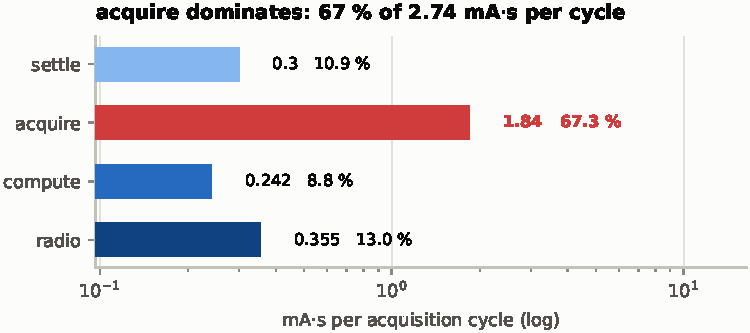
\includegraphics[width=0.84\textwidth]{kit_ra8d1_energy.pdf}
  \\[2mm]
  \begin{columns}[T]
    \begin{column}{0.49\textwidth}
      \scriptsize
      Acquisition dominates, as on every MEMS kit here. Compute is 8.8 \% ---
      three times a single-axis kit's share, and still small. Radio 13 \%, also
      $3\times$: three frames per acquisition.
    \end{column}
    \begin{column}{0.49\textwidth}
      \scriptsize\color{pdmcrit}
      \textbf{The model was wrong until this branch.} It used a flat 1000 ms
      ``standard acquisition'' for every kit while the firmware acquires 8192
      samples at 26.667 kHz $=$ 307 ms --- a $3.3\times$ error in the largest
      term, already quoted in four pushed READMEs.
      \par\color{pdmink2}
      Now derived from \texttt{acq\_samples / fs\_hz}, with a property test
      asserting it matches \texttt{app\_config.h}.
    \end{column}
  \end{columns}
  \srcnote{\nolinkurl{tools/power_budget.py}; corrected shares ---
  stwinbx1 85.0\,\%\,$\rightarrow$\,63.5\,\%, alif\_e7
  86.8\,\%\,$\rightarrow$\,66.9\,\%, ra8d1 87.0\,\%\,$\rightarrow$\,67.3\,\%.
  Battery-life figures moved by under 3 \%, because self-discharge dominates
  the load on four of the five kits --- the conclusions survive, the
  percentages did not.}
\end{frame}

% ------------------------------------------------------- order tracking: the --
\begin{frame}{Order tracking: the design's assumption was wrong}
  \centering
  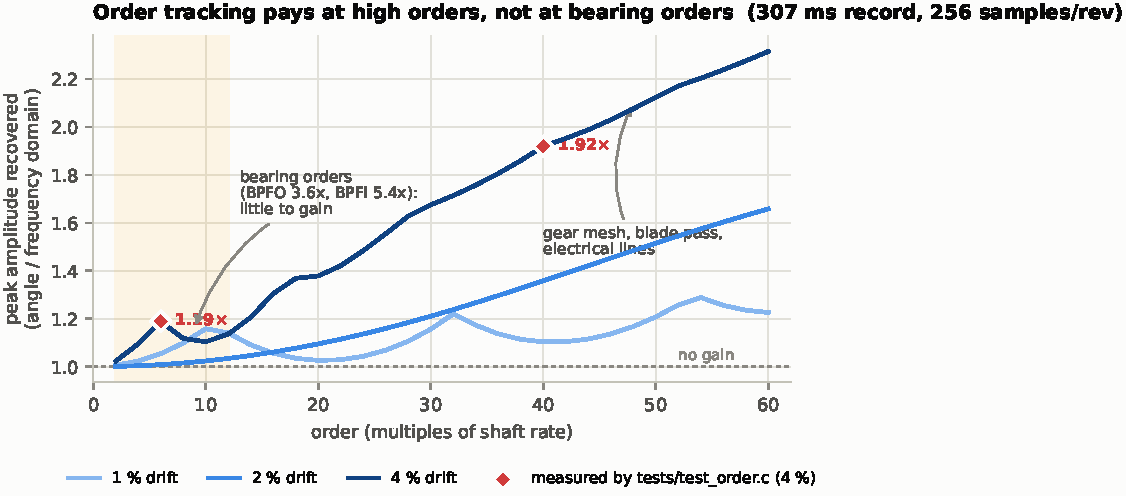
\includegraphics[width=0.70\textwidth]{ra8d1_order_gain.pdf}
  \\[1mm]
  \begin{columns}[T]
    \begin{column}{0.49\textwidth}
      \scriptsize
      Smearing goes as (order $\times$ drift $\times$ record length). At a
      307 ms record the bins are 3.26 Hz and a 6x line at 4 \% drift smears
      over $\sim$7 Hz --- barely wider than a Hann main lobe.
      \\[2mm]
      \textbf{So resampling is nearly pointless at bearing orders here.} The
      module's own docstring claimed 8--10 dB. The test said 1.5 dB.
    \end{column}
    \begin{column}{0.49\textwidth}
      \scriptsize\color{pdmink2}
      It pays where an analyst actually fights: gear mesh, blade pass,
      electrical lines. At order 40 the same drift costs 5.67 dB and
      resampling returns $1.92\times$.
      \\[2mm]
      The red markers are the C test's measured values, parsed from its own
      output by the figure script --- so the figure cannot quietly drift away
      from the test it illustrates.
    \end{column}
  \end{columns}
  \srcnote{\nolinkurl{hardware/ra8d1/tests/test_order.c} --- 14 checks.}
\end{frame}

\begin{frame}{The same line, both domains}
  \centering
  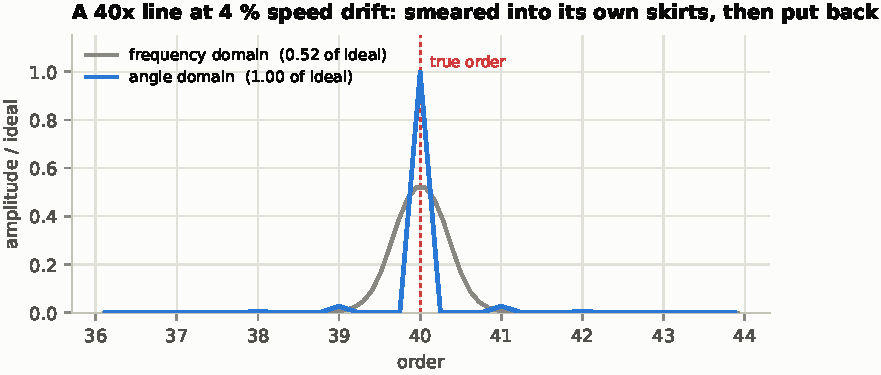
\includegraphics[width=0.74\textwidth]{ra8d1_order_spectrum.pdf}
  \\[2mm]
  \begin{columns}[T]
    \begin{column}{0.49\textwidth}
      \scriptsize
      A 40x line at 4 \% drift: 0.52 of ideal amplitude spread over six bins,
      restored to 1.00 in one bin.
      \\[2mm]
      A trend built on the smeared peak tracks the VFD's duty cycle rather
      than the machine's condition --- a false alarm every time production
      changes speed.
    \end{column}
    \begin{column}{0.49\textwidth}
      \scriptsize\color{pdmink2}
      \textbf{An unlooked-for result.} On a \emph{perfectly steady} shaft the
      frequency domain still loses 1.16 dB, because the line falls between
      bins. Scallop loss.
      \\[1mm]
      The angle domain puts it exactly on an order bin. For amplitude-based
      trending --- most of ISO 20816 practice --- that is arguably worth more
      than the smearing recovery.
    \end{column}
  \end{columns}
\end{frame}

% --------------------------------------------------------------- three axes ---
\begin{frame}{Three axes on one wire format}
  \begin{columns}[T]
    \begin{column}{0.52\textwidth}
      \scriptsize
      One FIFO burst, three pipeline runs, three frames. The channel lives in
      \textbf{flag bits 8--9}, which were previously always zero --- so every
      single-axis kit's frames are byte-identical and the schema version does
      not move.
      \\[2mm]
      What the shared loop guarantees:
      \begin{itemize}\itemsep1pt
        \item one burst, so the axes are the \emph{same instant};
        \item sequence per \emph{frame} --- ingest deduplicates on
              (device, sequence), so a shared sequence would discard two of
              three;
        \item channel 0 alone drives the alarm state machine;
        \item an overrun costs \emph{one} frame, not three.
      \end{itemize}
    \end{column}
    \begin{column}{0.44\textwidth}
      \scriptsize\color{pdmcrit}
      \textbf{Two bugs, both plausible-and-wrong.}
      \par\color{pdmink2}
      \textbf{1.} The shared loop powers the sensor down as soon as channel 0's
      burst is in RAM. Both boards checked ``is the sensor powered?'' \emph{before}
      serving the cached channels, so axes 1 and 2 returned \texttt{NOT\_READY}
      and the node shipped \textbf{one} frame per acquisition --- correct
      features, correct flags, healthy-looking dashboard.
      \\[1mm]
      \textbf{2.} Power-down cleared the retained block, so the extra axes would
      have re-read the sensor: three different instants.
      \\[1mm]
      Both found on the first run of the three-axis end-to-end test.
    \end{column}
  \end{columns}
  \takeaway{The multi-channel path went into the \emph{shared} loop, guarded by
  \texttt{APP\_N\_AXES}, so single-axis builds emit identical bytes and
  1\,113 golden checks stay meaningful.}
\end{frame}

% ------------------------------------------------------------------- timing ---
\begin{frame}{Compute is 1.4 \% of the sensing window}
  \centering
  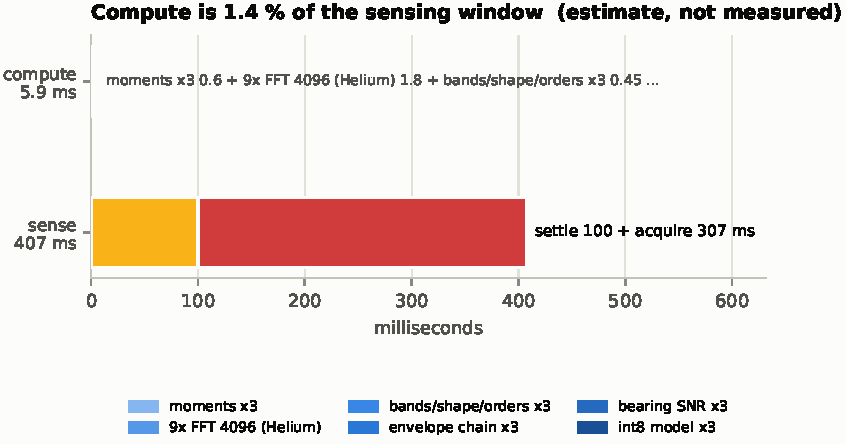
\includegraphics[width=0.86\textwidth]{kit_ra8d1_timing.pdf}
  \\[2mm]
  \begin{columns}[T]
    \begin{column}{0.49\textwidth}
      \scriptsize
      5.9 ms for three axes plus a 0.9 ms resampling pass, against a 407 ms
      sensing window. There is room for a 16384-point FFT (1.63 Hz envelope
      resolution), several bearings per node, or cyclostationary analysis ---
      none of which fit on a 256 kB part.
    \end{column}
    \begin{column}{0.49\textwidth}
      \scriptsize\color{pdmcrit}
      \textbf{The review item no test can catch.}
      \par\color{pdmink2}
      \texttt{-mfpu=fpv5-sp-d16} compiles, links, produces bit-identical
      numbers and passes every test in this repository, while running the FFT
      about twice as slow --- it hides the vector unit.
      \\[1mm]
      Only a disassembly tells you whether Helium was reached. Estimates on
      this slide are cycle counts, not measurements.
    \end{column}
  \end{columns}
\end{frame}

% --------------------------------------------------------------- honest gap ---
\begin{frame}{What it does not do}
  \begin{columns}[T]
    \begin{column}{0.52\textwidth}
      \scriptsize
      \textbf{The node does not ship order-domain features.}
      \\[1mm]
      \texttt{pdm\_pipeline\_run} takes its sample rate from
      \texttt{app\_config.h} at compile time. Feeding it a resampled record
      would label orders as hertz --- numbers that look right and are wrong by
      whatever the speed happened to be.
      \\[2mm]
      So the node instead:
      \begin{itemize}\itemsep1pt
        \item flags \texttt{SPEED\_UNSTEADY}, so the cloud widens its harmonic
              tolerance and discounts high orders;
        \item requests a raw snapshot, so the cloud does the angle-domain work;
        \item computes the local order spectrum anyway, for sites with no
              snapshot bandwidth.
      \end{itemize}
      \vspace{1mm}\par
      It deliberately does \textbf{not} set \texttt{ORDER\_TRACKED}: claiming
      the angle domain while shipping hertz is worse than no flag.
    \end{column}
    \begin{column}{0.44\textwidth}
      \scriptsize
      \begin{tabular}{@{}ll@{}}
        \toprule
        Shared DSP vs Python      & 1\,113 checks \\
        Resampling measured       & 14 checks \\
        Three-axis path end-to-end& 4 tests \\
        Config properties         & 19 tests \\
        Driver under \texttt{-Werror} & stub FSP \\
        \midrule
        Compiled for M85          & \textcolor{pdmcrit}{no} \\
        Flashed                   & \textcolor{pdmcrit}{no} \\
        Helium verified           & \textcolor{pdmcrit}{no} \\
        Timing measured           & \textcolor{pdmcrit}{no} \\
        Current measured          & \textcolor{pdmcrit}{no} \\
        Tacho on a rotor          & \textcolor{pdmcrit}{no} \\
        \bottomrule
      \end{tabular}
      \\[2mm]
      \scriptsize\color{pdmink2}
      Three files are referenced by the build and not written. They are listed
      rather than stubbed, so the gap is a link error --- not a function that
      returns success.
    \end{column}
  \end{columns}
\end{frame}

% ----------------------------------------------------------------- verdict ----
\begin{frame}{When to choose this part}
  \begin{columns}[T]
    \begin{column}{0.49\textwidth}
      \scriptsize
      \textbf{Choose it for} a VFD-driven critical asset where one radial
      channel is not enough: a gearbox where the mesh order matters, a fan
      where blade pass matters, a compressor whose duty varies through the day.
      \\[2mm]
      It costs more than the STWIN, draws more current, and needs wiring the
      STWIN does not. It buys an axial channel, a \emph{measured} shaft speed,
      amplitude-accurate order analysis, and an order of magnitude of DSP
      headroom.
    \end{column}
    \begin{column}{0.49\textwidth}
      \scriptsize\color{pdmink2}
      \textbf{Do not choose it for} a non-VFD motor-pump set with one
      accessible bearing. There the STWIN is the better engineering choice at
      two-thirds the price, with the sensor and radio already on the board, and
      this part is over-specified.
      \\[2mm]
      That is the honest recommendation, and the reason both branches exist.
    \end{column}
  \end{columns}
  \takeaway{The tachometer, not the clock speed, is what makes this kit
  different --- and the measurement showed it pays at gear orders, not at
  bearing orders.}
\end{frame}

\end{document}
